\section{Simulation Analysis}
\label{sec:simulation}

\subsection{Initial Input}

%Introduzir a cena do ngspice costume
%Mostrar a cena optimizada e explicar o porque de termos usado estes valores diferentes

\indent

This section discusses the circuit simulation, performed using {\it Ngspice}. 

This circuit was entered into the {\it Ngspice} simulation environment. This tool is used to simulate analog electronic circuits and predict circuit behaviour. 
This {\it Ngspice} simulation begins by defining the base circuit, visible on image \ref{fig:ngspiceCircuit}. The circuit can be subdivided into the following components:
 
\begin{itemize}
    \item Voltage source;
    \item Transformer;
    \item Envelope detector;
    \item Voltage regulator.
\end{itemize}

\begin{figure}[H]
    \centering
    \includegraphics[width = 0.8\linewidth]{FullCircuitFigure.pdf}
    \caption{{\it Ngspice} circuit}
    \label{fig:ngspiceCircuit}
\end{figure}

After having the base circuit description, the parameters have been chosen by trial and error. The final values are present on the following table (table \ref{tab:InputNGS}):

\begin{table}[H]
  \centering
  \begin{tabular}{|l|r|}
    \hline    
    {\bf Name} & {\bf Value} \\ \hline
    \input{../Analysis/InputParameters.tex}
  \end{tabular}
  \caption{Input Parameters}
  \label{tab:InputNGS}
\end{table}

With this process it was discovered that:
\begin{itemize}
    \item The number of winding of the transformer ($n$) was not changed a lot, this value was only to reduce the input voltage to a one with more manageable values. A higher $n$ means a lower voltage on the circuit (but a higher current).
    \item Increasing the Capacitor $C_1$ and the Resistor $R_1$, reduces the ripple and brings the voltage average slightly upwards;
    \item The number of diodes (on the voltage regulator) is directly responsible for the average voltage. The number of diodes changes the voltage at which the limiter cuts the current, this value is (approximately) the result from the product of $V_{ON}$ and the number of diodes in series;
    \item Changing the Value for the Resistor $R_2$ has a dramatic impact on the average voltage, a small increase, decreases the average voltage by a substantial amount. This was used to fine tune the average voltage without influencing the ripple very much.
\end{itemize}

Even though we want the best output possible, the price of the components has to be taken into consideration. 
The method utilised for optimising the output results was trial and error. The parameters were changed until the merit stopped increasing. This resulted in an expensive circuit, but with great results on the output.

\subsection{Results}

\indent

With the parameters honed in, the following graph (Figure \ref{fig:ngsOut}) is obtained, containing the voltage input and output on both the envelope detector and the voltage regulator:

\begin{figure}[H]
    \centering
    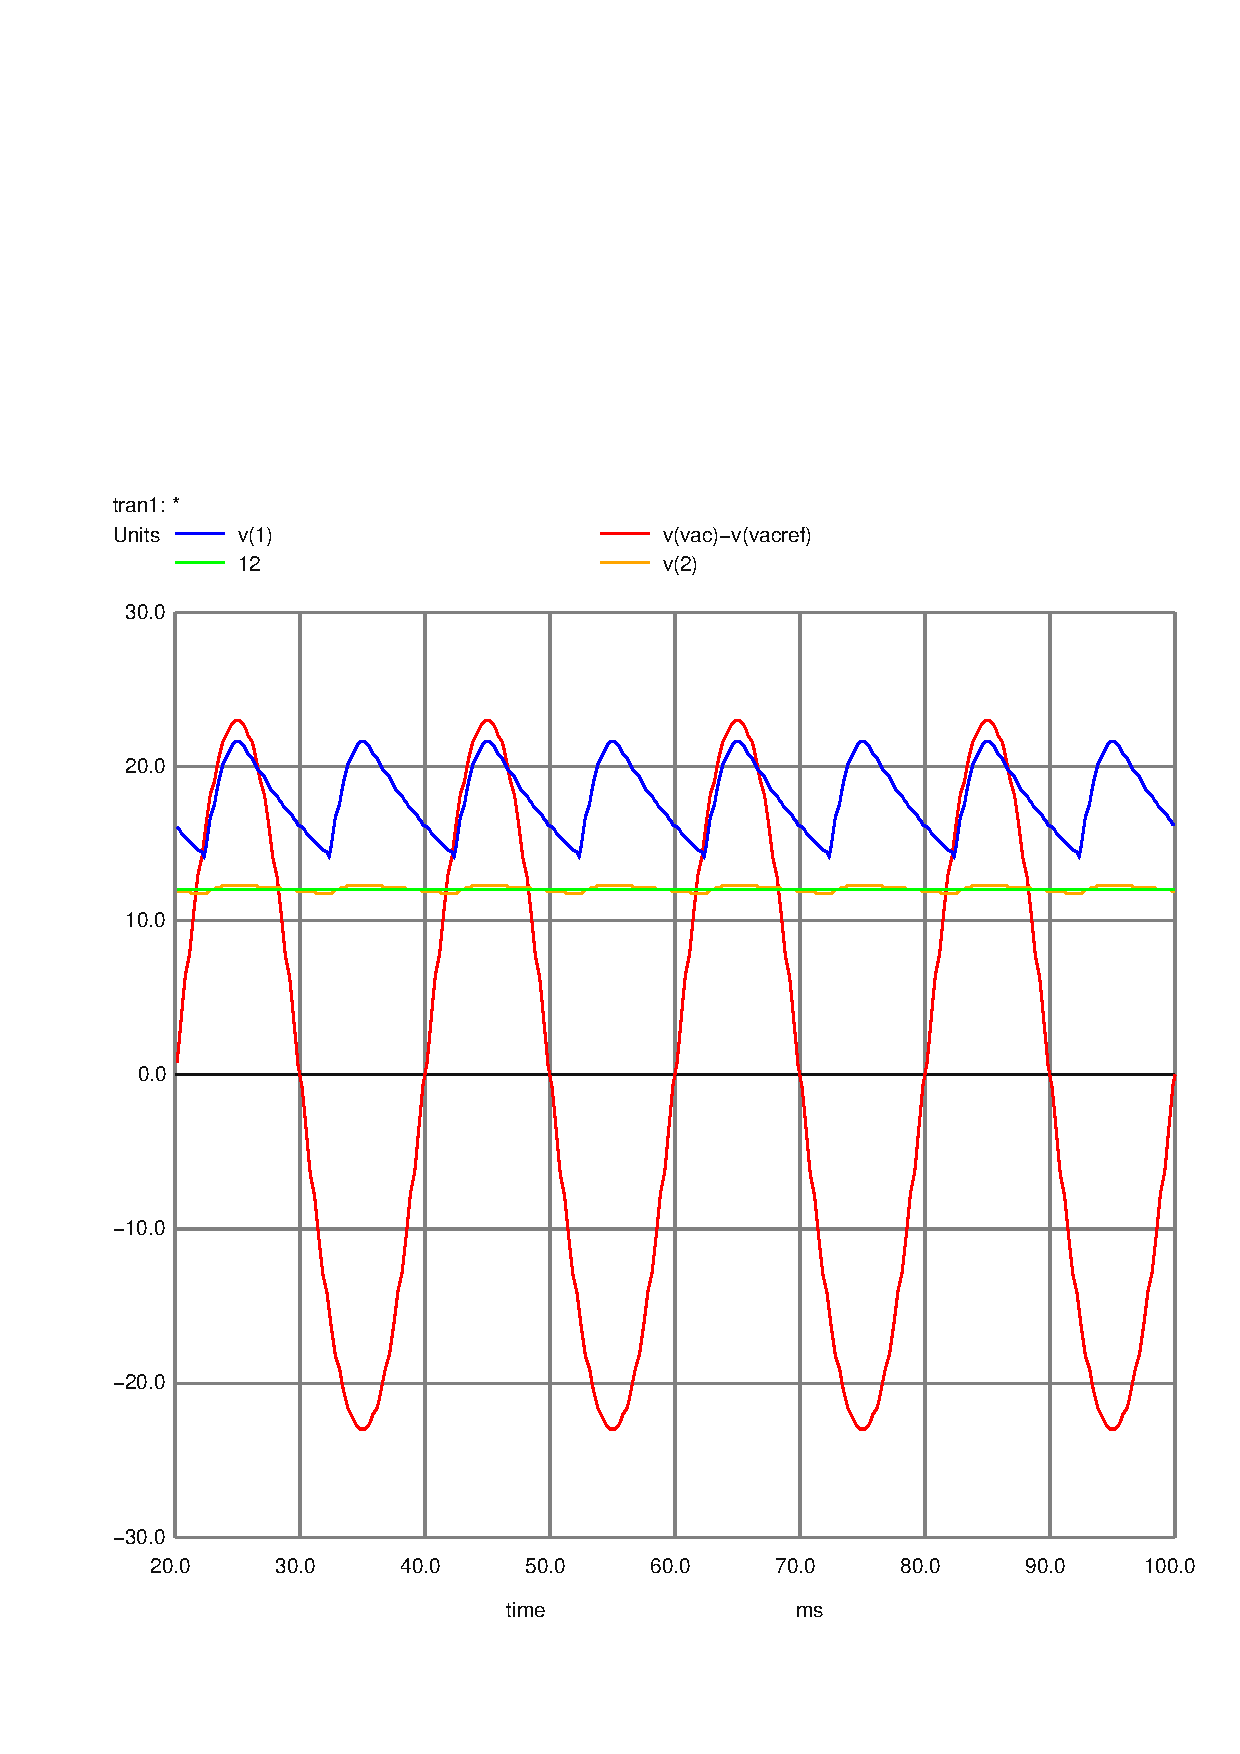
\includegraphics[width=.6\linewidth, trim={2cm 1.5cm 0.5cm 6cm}, clip]{../Simulation/sim1.pdf}
    \caption{{\it Ngspice} Output}
    \label{fig:ngsOut}
\end{figure}

Since the voltage ripple and the voltage deviation (from 12V) are what is going to be analysed, a closed up graph at these aspects was plotted (Figure \ref{fig:ngsOutClose}): 

\begin{figure}[H]
    \centering
    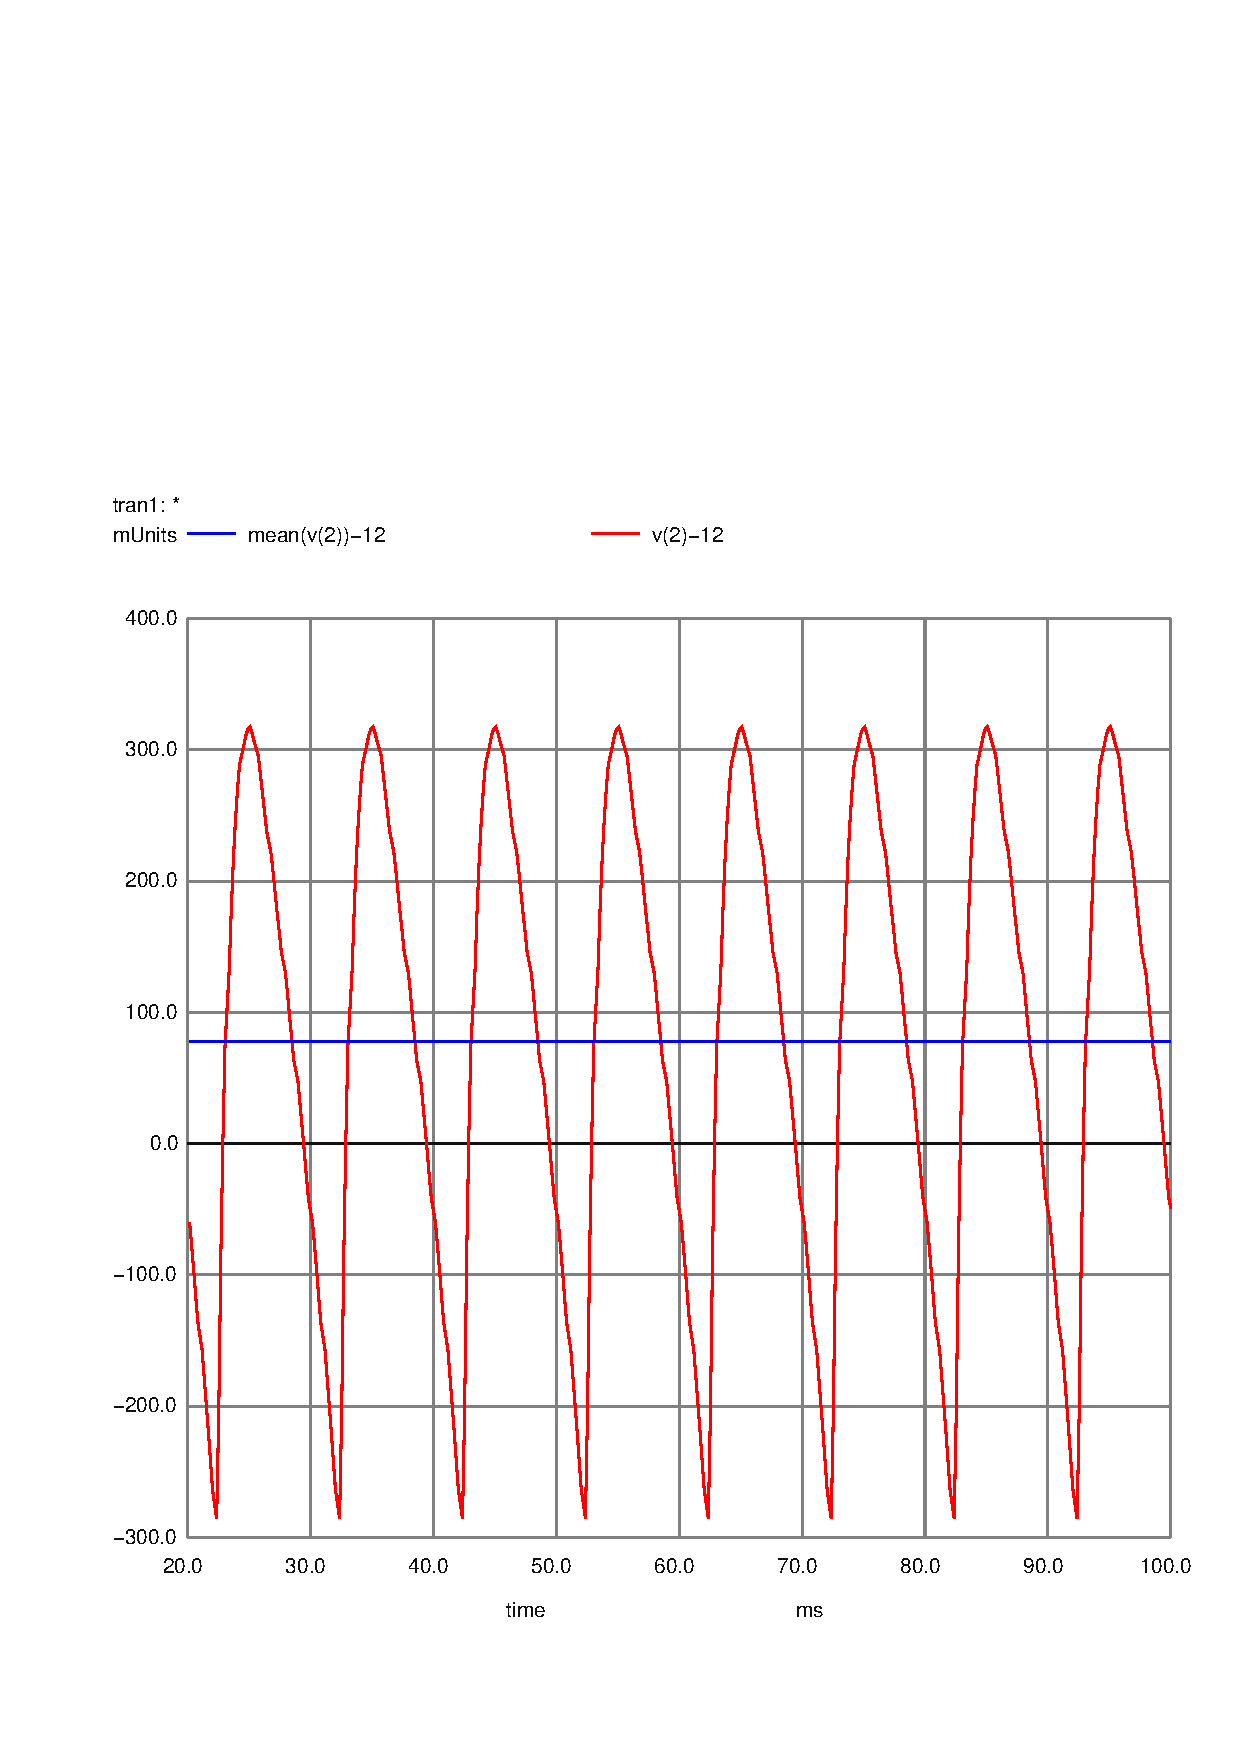
\includegraphics[width=.6\linewidth, trim={2cm 1.5cm 0.5cm 6cm}, clip]{../Simulation/sim2.pdf}
    \caption{{\it Ngspice} Output Close up}
    \label{fig:ngsOutClose}
\end{figure}



The quality of the output from this simulation can be analysed through the values shown in the next table (Figure \ref{tab:ngsOutParam}).

\begin{table}[H]
  \centering
  \begin{tabular}{|l|r|}
    \hline    
    {\bf Name} & {\bf Value} \\ \hline
    @c[i] & 0.000000e+00\\ \hline
@gcs[i] & -2.04136e-04\\ \hline
@r1[i] & 1.945229e-04\\ \hline
@r2[i] & -2.04136e-04\\ \hline
@r3[i] & -9.61363e-06\\ \hline
@r4[i] & 1.156284e-03\\ \hline
@r5[i] & 2.041365e-04\\ \hline
@r6[i] & 9.617613e-04\\ \hline
@r7[i] & 9.617613e-04\\ \hline
v(1) & 5.008942e+00\\ \hline
v(2) & 4.808960e+00\\ \hline
v(3) & 4.394159e+00\\ \hline
v(4) & 0.000000e+00\\ \hline
v(5) & 4.837862e+00\\ \hline
v(6) & 5.474755e+00\\ \hline
v(7) & -2.00872e+00\\ \hline
v(8) & -2.97092e+00\\ \hline

  \end{tabular}
  \caption{Output Parameters}
  \label{tab:ngsOutParam}
\end{table}


As it can be seen, the ripple as well as the mean voltage average have values which are very close to 0. However, in order to reach those values expensive components are needed, thus the high value for the cost ($mu$). Since the rate at which the ripple and the mean voltage average decreased was higher than the rate at which the cost ($mu$) increased, a high merit value was obtained.



